\documentclass[crop=false,10pt,ngerman]{standalone}
\usepackage{standard}

\usepackage[pages=some]{background}
\backgroundsetup{
  scale=0.8,
  opacity=0.3,
  angle=90,
  contents={%
    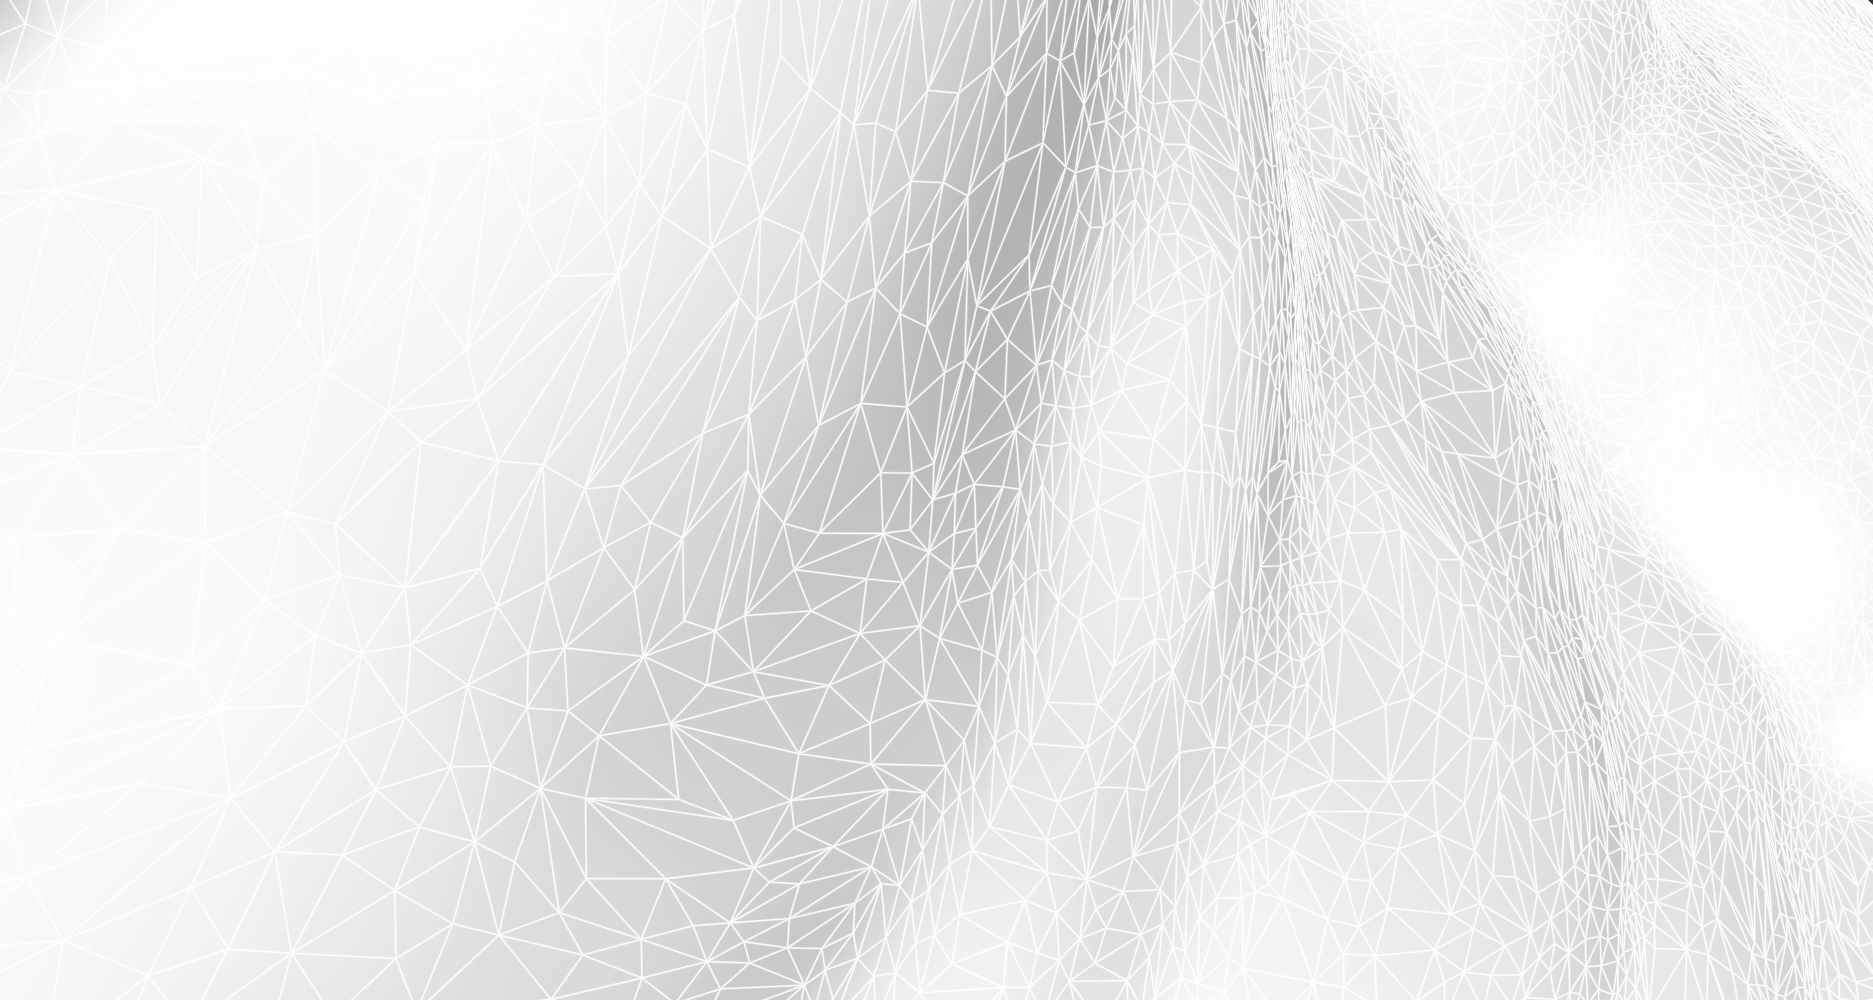
\includegraphics{images/background.png}
  }
}

\begin{document}

  \begin{titlepage}
    \BgThispage
    \newgeometry{top=0mm,bottom=0mm,right=20mm,left=50mm}
    \hbox{
      % \hspace*{0.2\textwidth}
      \rule{1pt}{\textheight}
      \hspace*{0.1\textwidth}
      \parbox[b]{0.75\textwidth}{
        {%
          Friedrich Schiller University Jena
        }\\
        {%
          Faculty of Mathematics and Computer Science
        }\\[2\baselineskip]
        {%
          \noindent\Large\bfseries%
          \linespread{1.3}%
          Design and Implementation of an \\[0.3\baselineskip]
          Efficient and Robust Algorithm for \\[0.3\baselineskip]
          Smoothing Curves on Surface Meshes
          % \\[0.3\baselineskip]
          % for the Application in a Medical Context
        }\\[2\baselineskip]
        {%
          \large%
          \textsc{Master's thesis} \\[\baselineskip]
          \textit{%
            for obtaining the academic degree \\[0.5\baselineskip]
            Master of Science (M.Sc.) in Mathematics
          }
        }\\[3\baselineskip]
        {%
          \large%
          \textrm{submitted by Markus Pawellek}
        }\\[2\baselineskip]
        {%
          born on May 7th, 1995 in Meiningen \\
          Student Number: 144645
        }\\[3\baselineskip]
        \begin{tabular}{ll}
          \large First Supervisor: & \large Kai Lawonn \\
          \\
          \large Second Supervisor: & \large Noeska Smit \\
          \\
          \large Third Supervisor: & \large Hauke Bartsch
        \end{tabular}\\[3\baselineskip]
        \vspace{0.1\textheight}
        {%
          Jena, \today
        }
        \vspace{0.08\textheight}
      }
    }
    \restoregeometry
  \end{titlepage}

\end{document}
